\chapter{影响社会认知的障碍:自闭症谱系障碍} \label{chap:chap62}

精神发育迟滞,现在被广泛称为智力障碍,目前被定义为智商低于 70 并伴有明显的适应功能缺陷。
这两个术语已被广泛用于标记与产前或产后早期大脑异常相关的各种认知障碍。
几十年来,患有罕见智力障碍综合征(例如 Rett 综合征或脆性 X 综合征)的个体亚群的特征在于其遗传病因。
我们现在开始阐明更普遍的神经发育障碍的复杂遗传学,这些障碍没有区分它们的明显物理特征,包括所谓的自闭症谱系障碍 (ASD) 的特发性或非综合征形式。
对罕见遗传综合征的深入研究所产生的见解与揭示特发性 ASD 潜在遗传学的成功相结合,已经改变了我们对人类大脑正常和病理发育的理解。


所有这些疾病的共同点是终生持续存在的精神障碍,阻碍了发展和学习。
一般来说,即使所有的心理功能似乎都受到影响,也可以区分具有不同病因和自然历史的情况,因为一些认知领域往往比其他认知领域受损更严重。
事实上,这些差异在诊断方案中得到了体现,这些方案区分了主要影响一般认知、社会认知或知觉的发育异常。
这些不同的认知和行为弱点可能为了解正常发育中特定心理功能的起源和发育时间过程提供有用的线索。


在本章中,我们主要关注包括社会功能异常在内的神经发育障碍,包括自闭症谱系障碍、脆性 X 综合征、威廉姆斯综合征、雷特综合征以及 Angelman 和 Prader-Willi 综合征。
这些情况都会损害高度复杂的大脑功能,包括社会意识和沟通。
ASD 成为主要关注点有几个原因:
遗传风险与其他常见神经精神疾病(包括精神分裂症)的重叠;
以及缺乏明确的神经病理学。
它们也是许多精神综合征常见的病因学和表型异质性的范例。
在这方面,ASD 是一种典型的神经精神综合征。



\section{自闭症谱系障碍表型具有共同的行为特征}

严重的社会障碍可能一直伴随着我们,但将自闭症定性为一种医学综合症最早是在 1943 年由 Leo Kanner 和 1944 年由 Hans Asperger 在文献中描述的。
今天,临床医生和研究人员将自闭症视为具有两个定义但高度可变的诊断特征的一系列障碍:
社交沟通障碍和兴趣高度受限的刻板行为。


直到最近,“阿斯伯格综合症”一词还用于描述满足这两个诊断标准但语言习得没有延迟且智商在正常范围内的人。
在最新版的标准精神病学诊断手册《精神疾病诊断和统计手册》第五版 (DSM-5) 中,阿斯伯格综合症以及一种称为广泛性发育障碍的独特疾病,未另行说明——旨在捕捉有缺陷的个体 在其他领域不符合完整标准的社交沟通中的人被淘汰,以支持在单个频谱结构中包含变化。


自闭症谱系障碍存在于至少 1.5\% 的人口中。
严格的流行病学研究估计,各种社会残疾的患病率高达 2.6\%,远高于几十年前的估计。
在相对较短的时间内流行率增加的原因引起了相当大的兴趣和激烈的争论,特别是在普通公众中。
在科学界,已经达成共识,即这种增加反映了诊断标准的变化、家庭和医疗保健专业人员意识的提高、“诊断替代”(以前被诊断为智力障碍的人现在更有可能 被确定为社会残疾),并且一些真正的发病率增加。
下面将就遗传风险讨论这些问题。


自闭症谱系障碍主要发生在男性中,尽管通常引用的 4:1 男女比例最近因担心用于确定诊断的方法(包括诊断仪器)中的男性偏见而受到质疑。
然而,即使考虑到这些挑战,累积的证据表明男性比例偏差至少为 2:1 至 3:1。
IQ 范围内的个人都会受到影响,并且根据当前的诊断实践,大约一半的 ASD 患者也有智力障碍。
根据定义,ASD 必须在 3 岁之前可以检测到,但最近的研究表明,可以在出生后的第一年内很好地识别出高风险家庭中受影响的儿童。
ASD 存在于所有国家和文化以及每个社会经济群体中。


尽管 ASD 明显影响大脑,但尚未确定明确的生物标志物;
因此,诊断基于行为标准。
这并不意味着没有很强的生物学相关性,包括特定的基因突变和神经影像学发现,但这些都没有足够的特异性或预测性,无法替代临床评估的黄金标准。
此外,由于行为在发育过程中是可变的,并且取决于许多因素——年龄、环境、社会背景以及补救帮助的可用性和持续时间——没有任何一种行为可能永远具有决定性的诊断意义。


与其他神经发育综合症一样,自闭症谱系障碍通常会持续一生。
然而,在最近的纵向研究中,大约 10\% 的明显受影响的儿童表现出改善,在以后的生活中很少或没有社交障碍的证据。
自闭症不是进行性的。
相反,特殊的教育计划和专业支持通常会随着年龄的增长而改善行为和适应功能。



\section{自闭症谱系障碍表型也有明显的认知异常}

\subsection{自闭症谱系障碍的社交沟通受损:心智失明假说}

一种社会交流的认知理论假设人类具有特别发达的能力,能够以直觉和全自动的方式理解他人的心理状态。
看着一个年轻人在没有钥匙的情况下偷偷地试图打开车门,你会立即明白她相信她可以在不被注意的情况下闯入,你希望她一发现有人在看就跑掉。
因此,你通过从她的明显行为推断她的心理状态(欲望、意图、信念、知识)来解释和预测她的行为。
这种所谓的心理化能力,被称为心智理论,被认为依赖于特定的大脑机制和社会认知背后的回路(图 \ref{fig:62_1})。
此外,据推测,自闭症患者的心智化受损,对社会发展产生深远影响。


\begin{figure}[htbp]
	\centering
	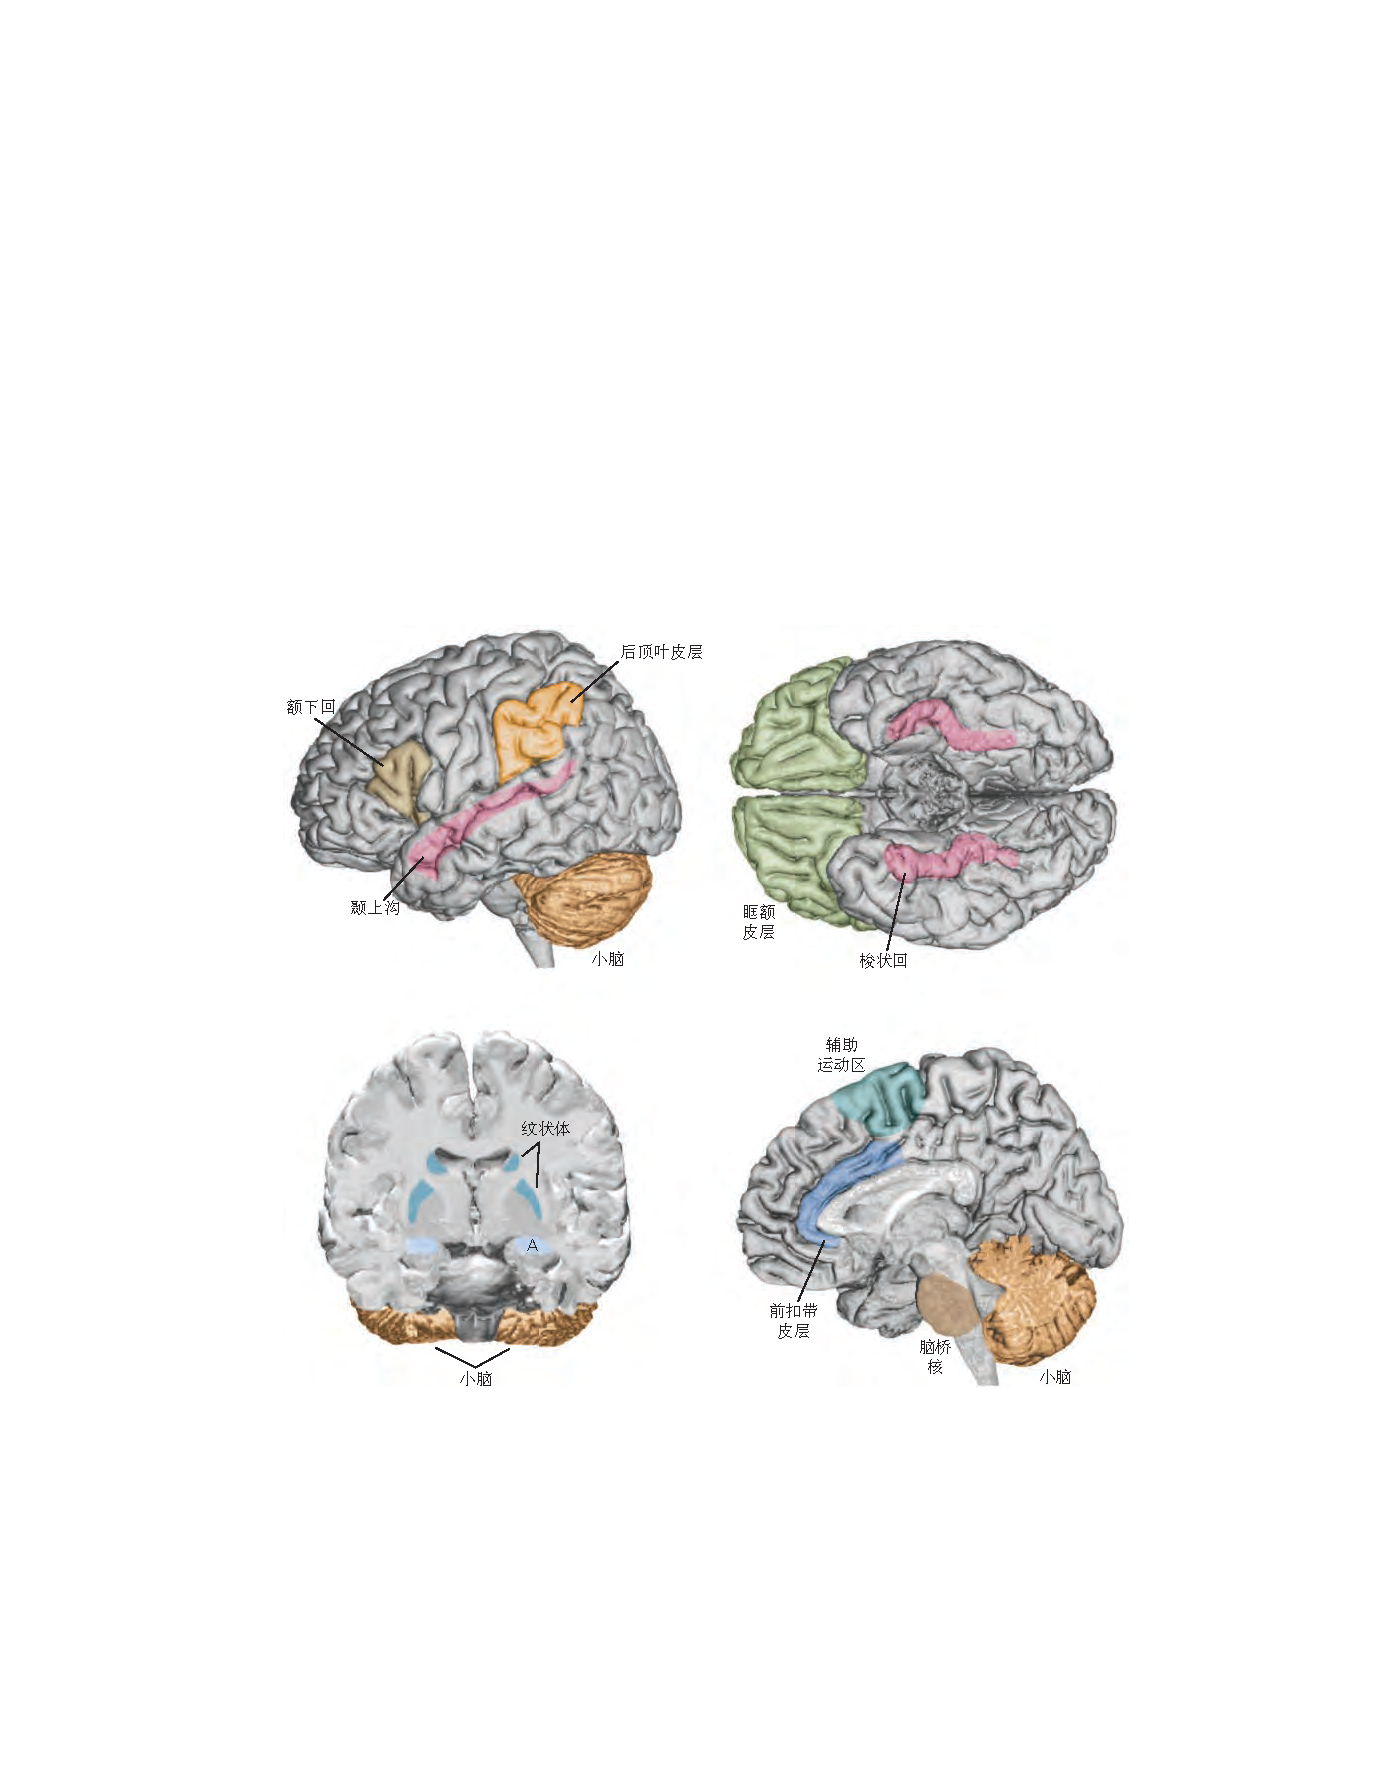
\includegraphics[width=0.8\linewidth]{chap62/fig_62_1}
	\caption{与自闭症的三个核心缺陷特征有关的大脑区域:社交互动受损、语言和交流受损以及重复和刻板行为的兴趣严重受限。 与社会缺陷有关的区域包括眶额皮质 (OFC)、前扣带皮层 (ACC) 和杏仁核 (A)。 与颞上沟 (STS) 接壤的皮质与调节生物正在移动的感知和注视感知有关。 面部处理涉及梭状回 (FG) 内的下颞叶皮层区域。 语言的理解和表达涉及许多区域,包括下额叶区域、纹状体和皮质下区域,例如桥脑核 (PN)。 纹状体也与重复行为的调节有关。 (缩写:IFG,额下回;PPC,后顶叶皮层;SMA,辅助运动区。)}
	\label{fig:62_1}
\end{figure}


现在普遍认为,洞察他人的心理状态取决于自发心智化的能力。
自发心智化让我们意识到不同的人有不同的想法,想法是内在的,不同于外在的现实。


无法心智化或“思维失明”首先使用简单的木偶游戏 Sally-Anne 测试对自闭症儿童进行了测试。
患有 ASD 的幼儿与患有唐氏综合症的儿童或通常发育中的 4 岁儿童不同,他们无法预测木偶在离开房间时首先会在哪里寻找被移动的物体。
他们无法想象木偶会“认为”物体会在木偶离开它的地方(图 \ref{fig:62_2})。
许多自闭症儿童最终确实学会了通过这项任务,但平均要延迟 5 年。
即使在成年后,如此缓慢获得的心智化仍然是费力和容易出错的。


\begin{figure}[htbp]
	\centering
	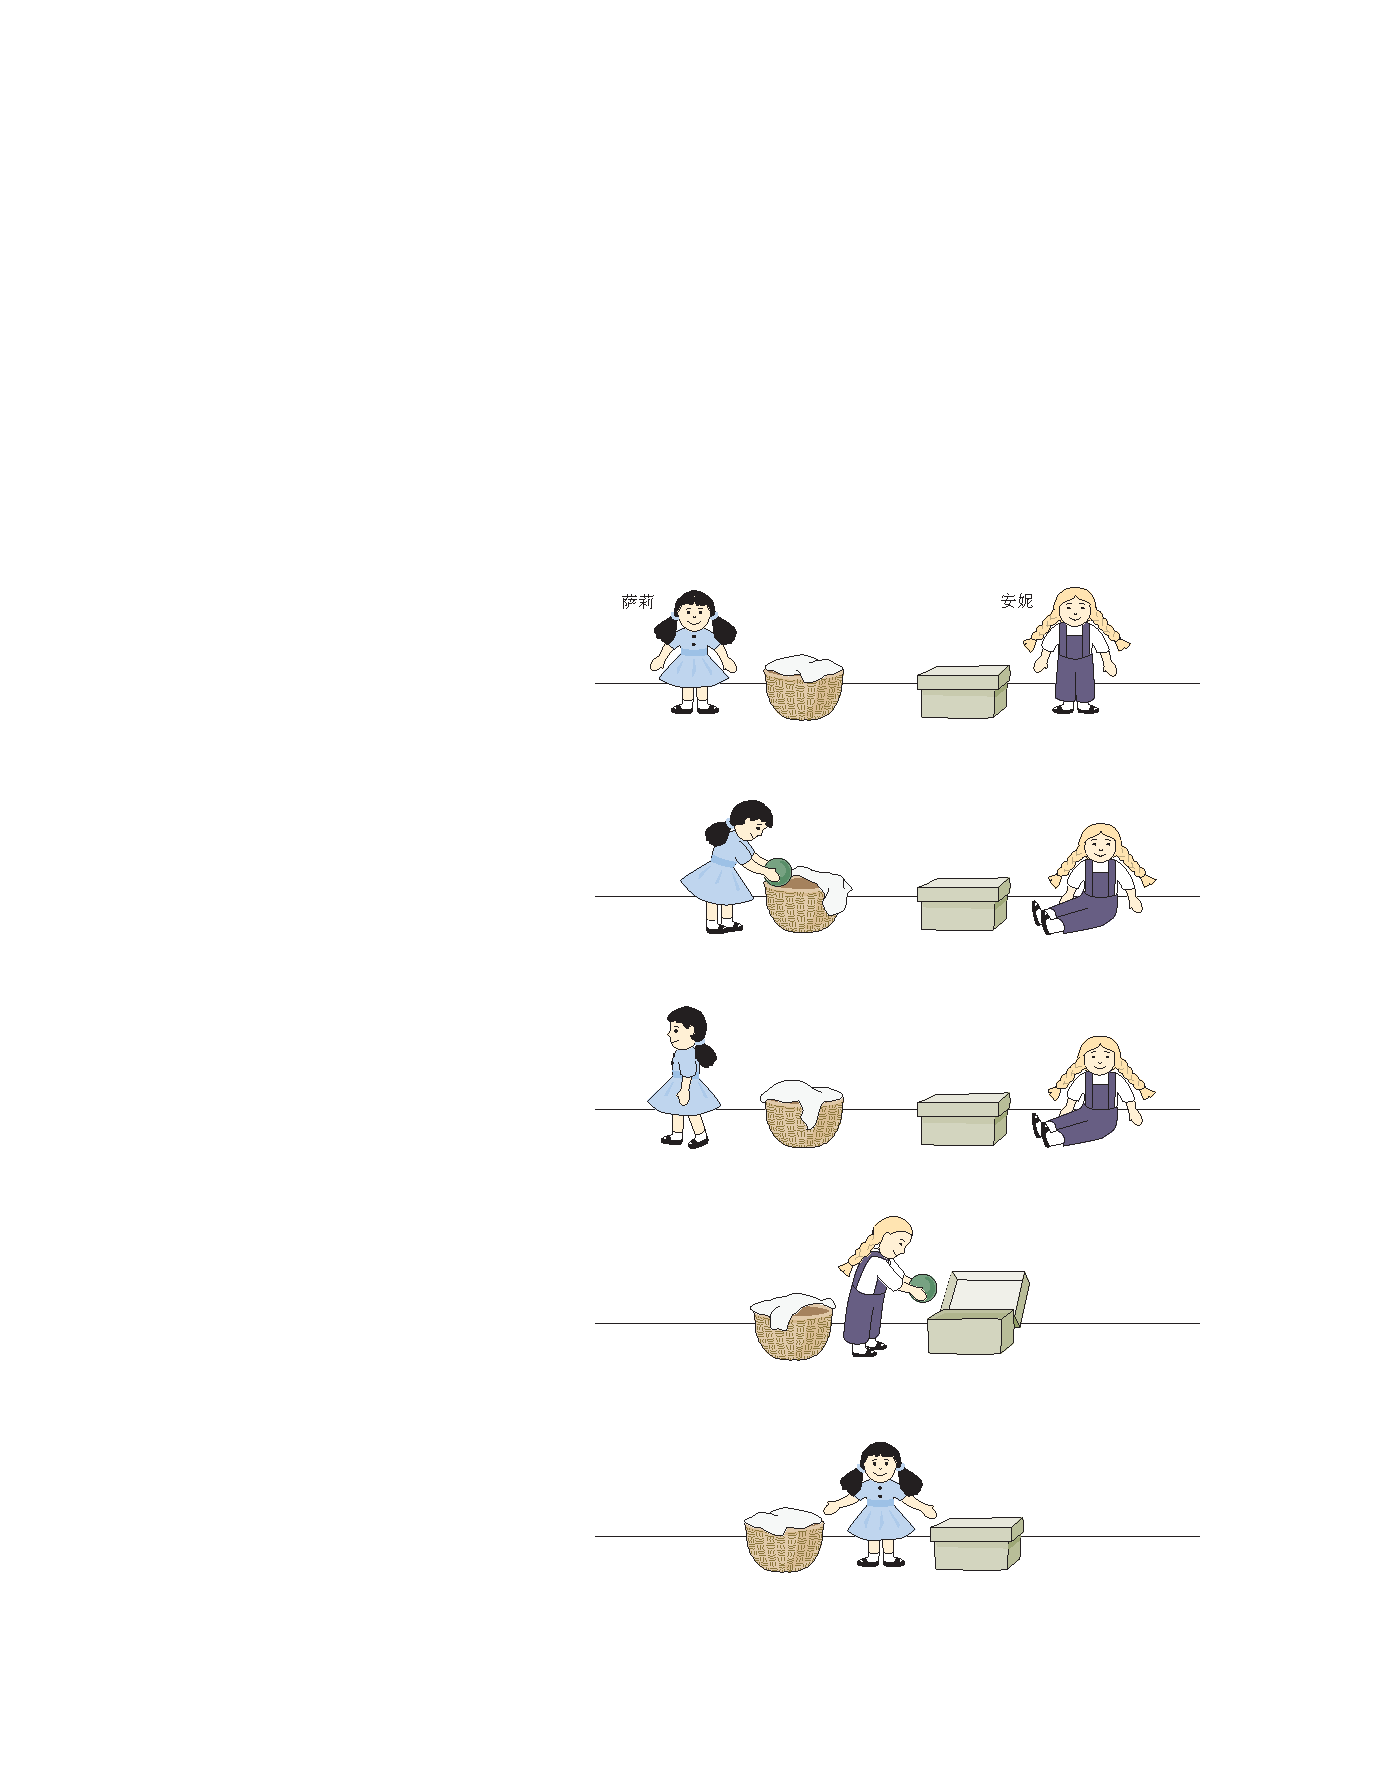
\includegraphics[width=0.65\linewidth]{chap62/fig_62_2}
	\caption{莎莉-安妮测试。 “心智理论”的第一次测试从使用两个玩偶的脚本表演开始。 莎莉有一个篮子; 安妮有一个盒子。 莎莉把一个球放进她的篮子里。 她去散步,然后离开了房间。 当莎莉在外面时,顽皮的安妮把球从篮子里拿出来放进了她的盒子里。 现在莎莉散步回来,想玩她的球。 她会在哪里寻找球、篮子或盒子? 答案是篮子,这对大多数发育正常的 4 岁儿童来说是显而易见的,但对智力年龄相同或更高的自闭症儿童而言则不然。 (改编自 Axel Scheffler 的原创作品。)}
	\label{fig:62_2}
\end{figure}


与此同时,患有自闭症谱系障碍的幼儿对身体原因和事件表现出极好的理解能力。
例如,一个无法谎报另一个箱子锁着的孩子很有能力锁上同一个箱子以防止里面的东西被偷走。


自 20 世纪 80 年代中期以来,Sally-Anne 测试和其他心智化任务的变体已被用于患有 ASD 的儿童和成人(图 \ref{fig:62_3})。


\begin{figure}[htbp]
	\centering
	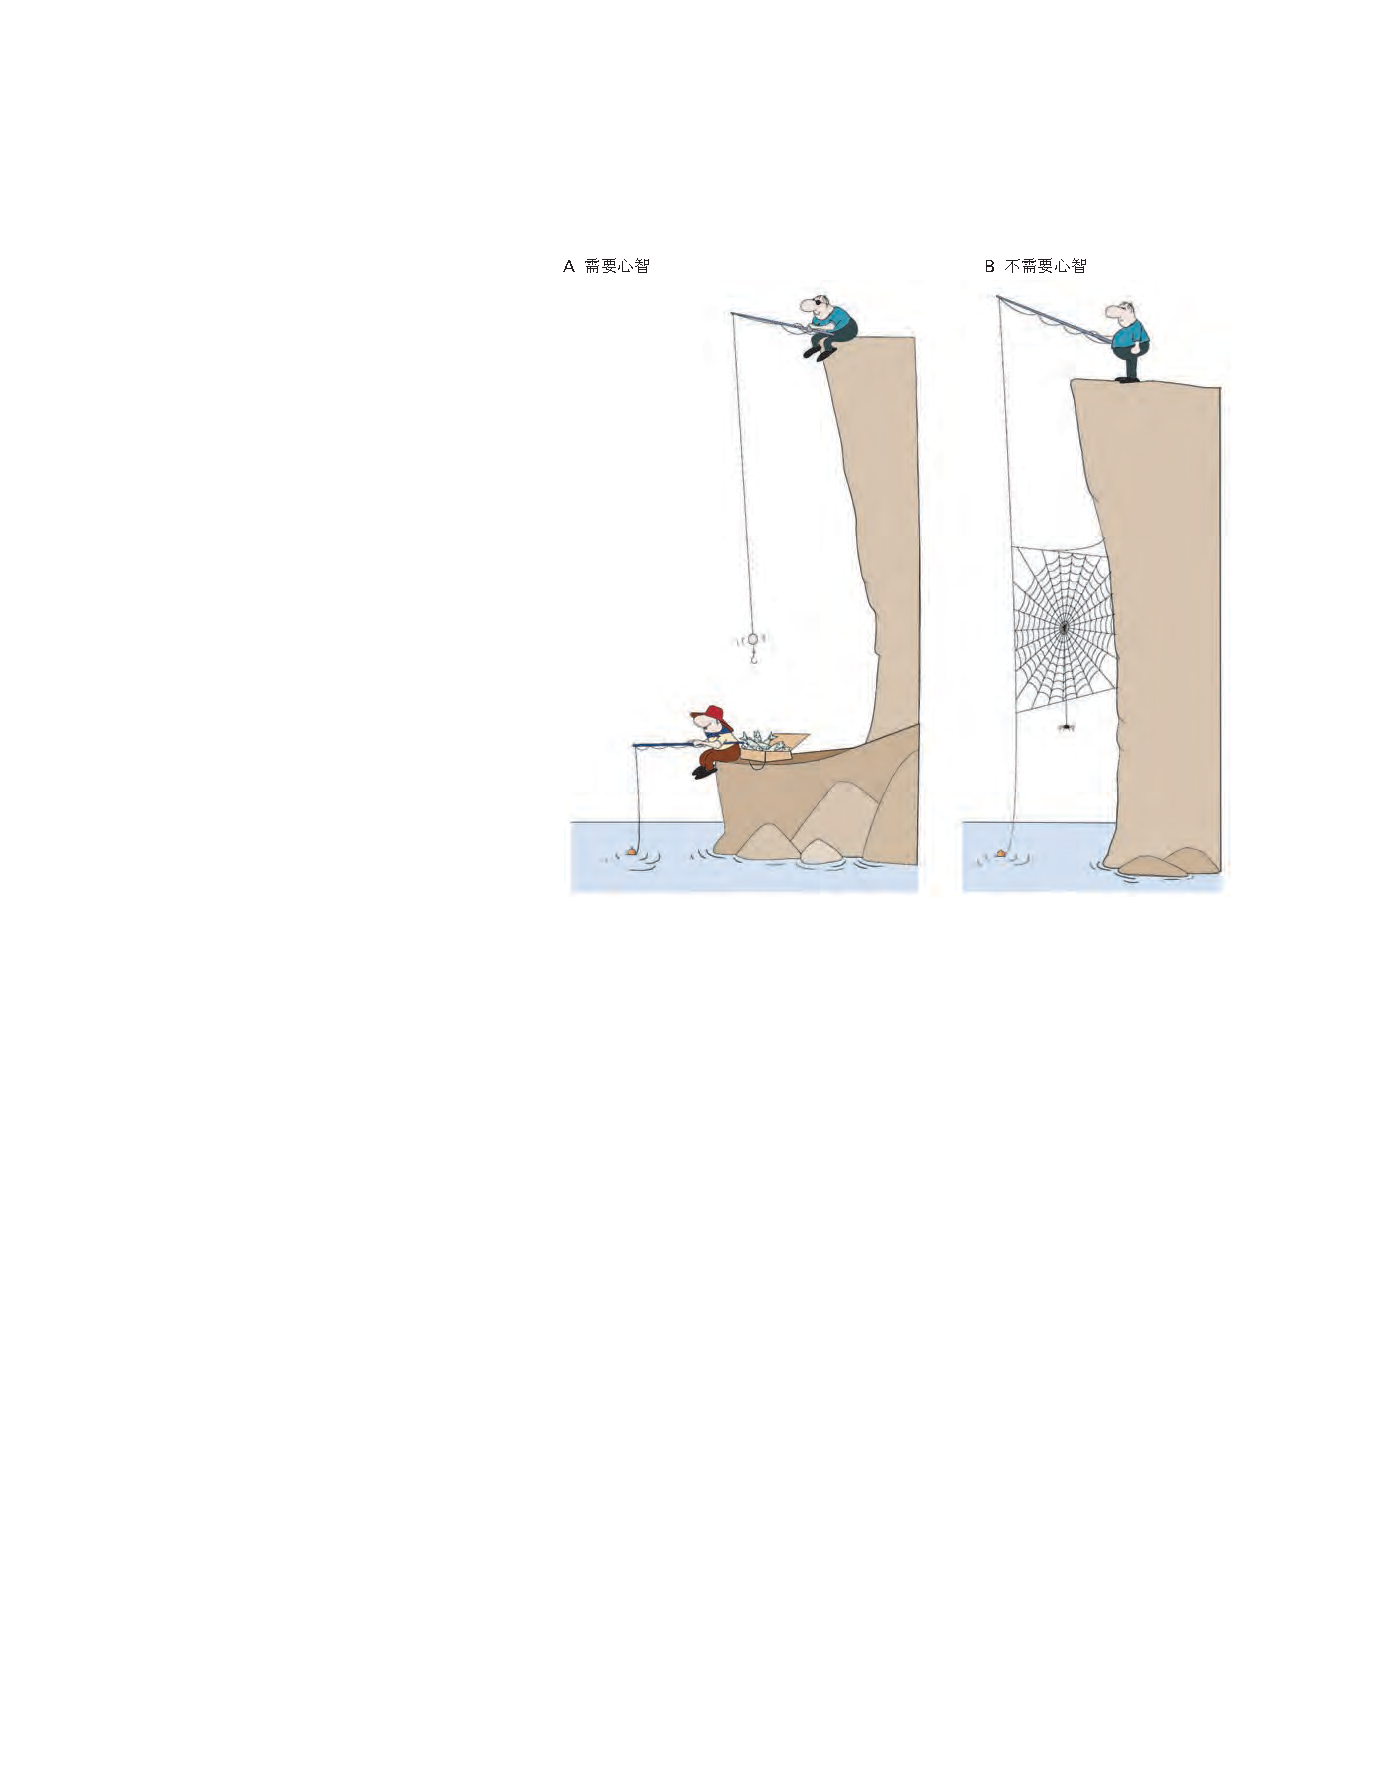
\includegraphics[width=0.7\linewidth]{chap62/fig_62_3}
	\caption{用于“心智化”成像研究的卡通示例。 要求参与者(静默地)考虑每张图片的含义,然后对其进行解释。 在一项功能性磁共振成像研究中,正常成年人被动观看需要心智化的卡通片和不需要心智化的卡通片。 每个受试者的大脑区域特征网络都被激活(见图 \ref{fig:62_4})。 (改编自 Gallagher 等人,2000 年。)}
	\label{fig:62_3}
\end{figure}


\begin{figure}[htbp]
	\centering
	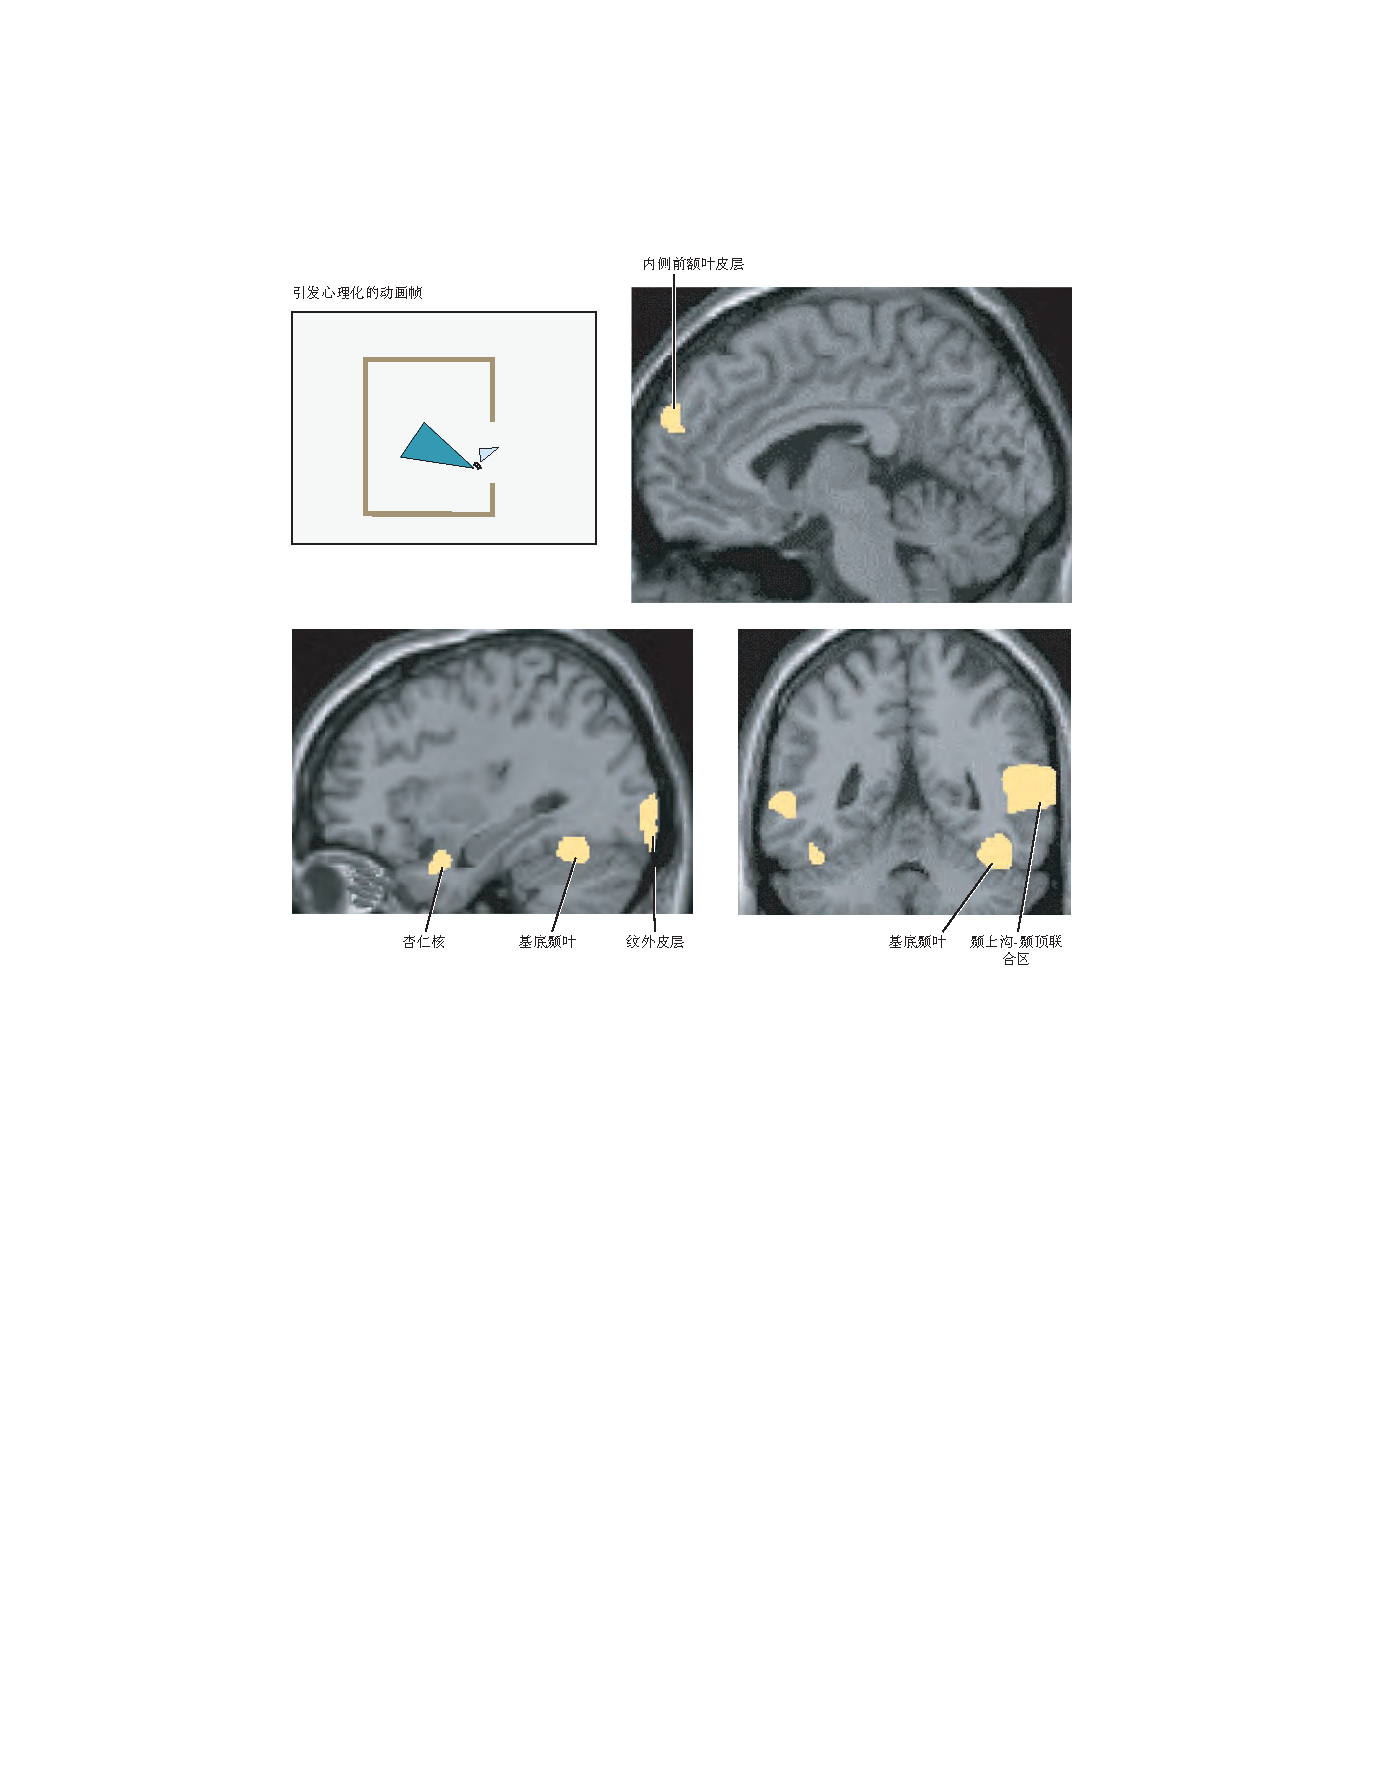
\includegraphics[width=0.75\linewidth]{chap62/fig_62_4}
	\caption{大脑的心智化系统。 向健康的志愿者展示动画三角形,这些三角形的移动方式使观众会将精神状态归因于他们。 在所示的示例框架中,较大的三角形被视为鼓励较小的三角形离开外壳。 他们还看到动画三角形,这些三角形或多或少以随机方式移动,因此不会引发心智化。 当比较这两种观察条件时,突出显示的区域显示大脑激活的正电子发射断层扫描扫描的差异。 (缩写:STS,颞上沟。)(经许可转载自 Castelli 等人,2002 年。版权所有 © 2002,牛津大学出版社。)}
	\label{fig:62_4}
\end{figure}


功能性神经成像已被用于检查健康受试者在从事需要思考精神状态的任务时的大脑活动。
这些研究中使用了广泛的使用视觉和语言刺激的任务。
在一项早期的正电子发射断层扫描研究中,对照组中的成年人观看了几何形状的无声动画。
在一些动画中,三角形在旨在唤起心智化的脚本场景中移动(例如,三角形互相欺骗)。
在其他动画中,三角形以一种不会引起心智化的方式随机移动。
比较受试者观看每种类型的动画时进行的扫描,揭示了一个由四个大脑中枢组成的特定网络,该网络涉及心智化(图 \ref{fig:62_4})。
使用相同动画的功能磁共振成像 (MRI) 研究表明,患有 ASD 的受试者在该网络中的活动减少了。


该网络有四个组件。
第一个位于内侧前额叶皮层,该区域被认为与监控自己的思想有关。
第二个组成部分位于颞上叶的颞顶区,已知会被眼睛注视和生物运动激活。
左半球这一区域有病变的患者无法通过 Sally-Anne 测试。
第三个区域是杏仁核,它参与评估社会和非社会信息以了解环境中的危险迹象。
第四个区域是涉及面孔感知的下颞区。


最近的研究使用旨在捕捉更细微和自然主义社会内容的刺激,例如,使用真实社会遭遇的电影而不是面部表情的静态图片。
这些研究已经确定了眼眶额叶皮层在社会认知中的作用。



\subsection{其他社会机制导致自闭症谱系障碍}

从出生开始,正常的婴儿就更喜欢注意人而不是其他刺激。
缺乏这种偏好可能会导致无法理解他人并与他人互动。
事实上,缺乏对社会刺激的优先关注和相互关注被广泛认为是 ASD 的早期迹象。
这些缺陷可能不涉及心智化问题,因为相互关注通常出现在第一年末,此时心智化迹象仍然很少。


长期以来,研究人员一直在考虑一种可能性,即特定的神经机制是对社会刺激(例如面部、声音和生物运动)的关注的基础。
支持这一假设的研究人员发现,患有 ASD 的人在观看社交场景时注视是异常的。
例如,多项研究发现,自闭症患者会注视他人的嘴巴,而不是表现出对眼睛的正常偏好(图 \ref{fig:62_5})。


\begin{figure}[htbp]
	\centering
	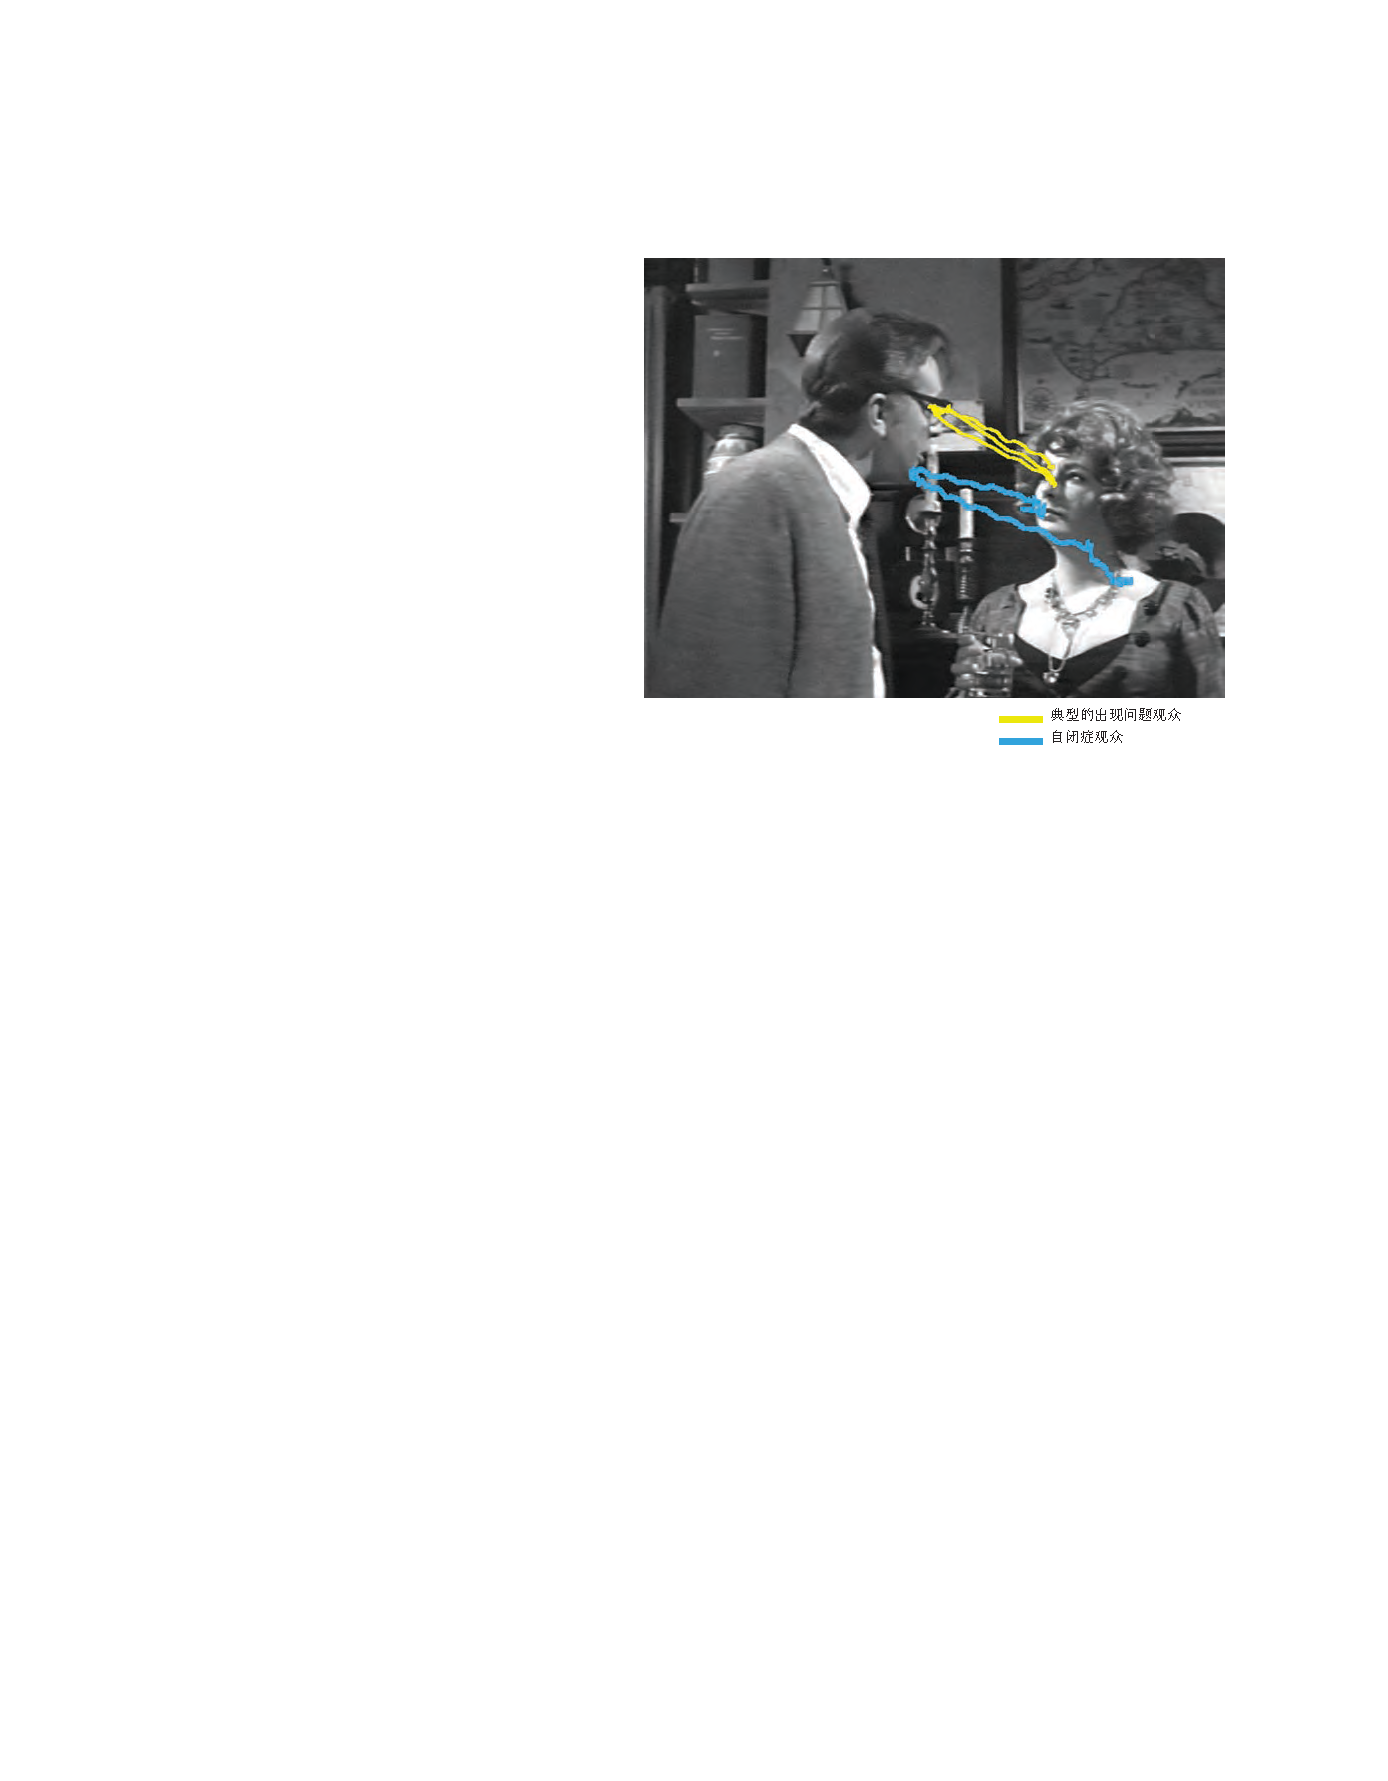
\includegraphics[width=0.65\linewidth]{chap62/fig_62_5}
	\caption{自闭症患者通常不会直视他人的眼睛。 当受试者观看电影《谁害怕弗吉尼亚狼》中的片段时,研究了自闭症患者的眼球运动模式? 在看人脸时,被摄者更倾向于看嘴巴而不是眼睛,在人与人之间激烈互动的场景中,他们更倾向于看无关紧要的地方而不是演员的脸。 (经许可转载自 Klin 等人,2002 年。版权所有 © 2002 美国精神病学协会。)}
	\label{fig:62_5}
\end{figure}



\subsection{自闭症患者缺乏行为灵活性}

ASD 中重复和僵硬的行为可能反映了额叶执行功能的异常,这是一系列更高级的认知过程,包括脱离给定任务的能力、抑制不适当的反应、坚持任务(计划和管理故意行为的顺序)、 在工作记忆中保留多项任务需求,监控性能,并将注意力从一项任务转移到另一项任务。


即使是智商在正常范围内的自闭症患者,在计划、组织和灵活切换行为方面也存在问题。
无论智商如何,受影响的人都难以提出单个物体的各种不同用途,例如手帕(用于阻挡打喷嚏、包裹松散的物体等)。
额叶获得性损伤的患者思维灵活度也较差。



\subsection{一些自闭症患者有特殊才能}

ASD 在某些个体中特别引人入胜的特征是“学者综合症”,其定义为存在一种或多种与个体的整体残疾形成鲜明对比但在一般人群中也很少见的特殊技能。
引用最广泛的估计是,10\% 的自闭症患者表现出这种非凡的能力,而其他形式的智力障碍患者中这一比例约为千分之一。


在迄今为止自我报告调查的最大 ASD 队列中(约 5,000 个家庭),据报道有 531 人在以下 10 个领域(按频率降序排列)具有特殊能力:音乐、记忆、艺术、阅读过度、数学、机械、协调、 方向、日历计算和超感官知觉。
随后的小规模研究表明,自闭症谱系障碍患者的学者技能流行率在 13\% 到 28\% 之间。


最近建立的学者综合症登记处现在包括来自 33 个国家的 400 多人。
根据家庭或看护者报告或自我报告,在一组 319 人中,他们符合某些标准并获得专家诊断,其中 75\% 在童年时期表现出专家技能的人被诊断为自闭症谱系障碍。
大约一半报告了一项特殊技能,一半报告了多项技能。
音乐是最常报告的特殊技能,其次是艺术、记忆和数学。
日历计算虽然与另一项技能一起出现在许多学者身上,但只有大约 5\% 的样本是唯一的技能。
在这个自我或家庭选择的群体中,总体性别分布反映了一般 ASD 的报告,男女比例约为 4:1。


对学者综合症的一种解释是,信息处理优先考虑微小的细节,而以看到更大的图景为代价。
(例如,图 \ref{fig:62_6} 中患有高功能自闭症的天才艺术家的绘画显示了非常详细的城市景观,以及详细的数字模式和日期。)一个类似的假设是涉及感知的大脑区域功能过度;
另一种可能性是,人们倾向于操纵符合严格框架的信息位,例如日历知识或公共汽车时刻表。
神经心理学数据支持这两种解释,但区分它们的决定性实验仍有待完成。


\begin{figure}[htbp]
	\centering
	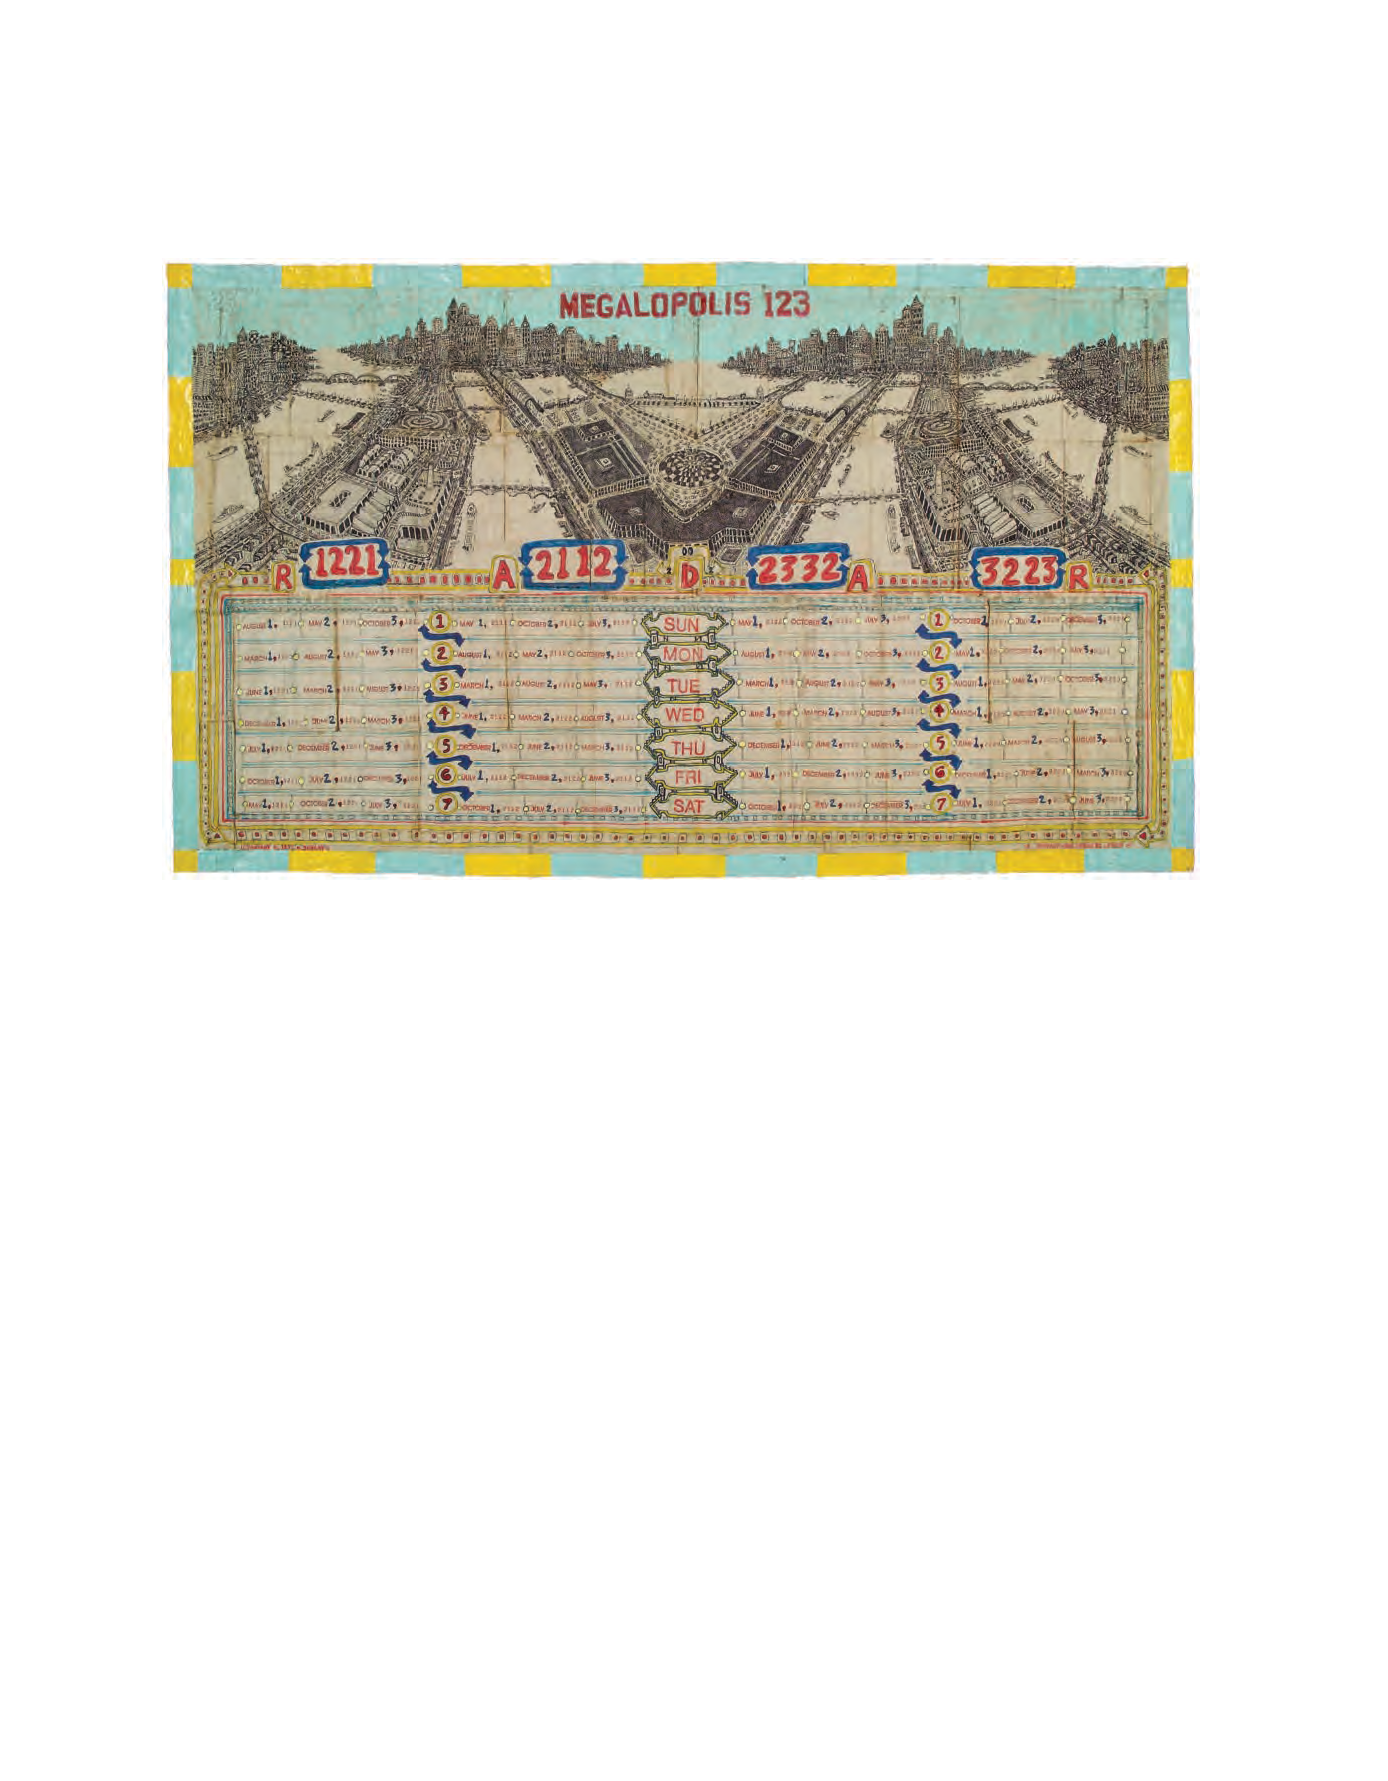
\includegraphics[width=0.9\linewidth]{chap62/fig_62_6}
	\caption{乔治·威德纳 (George Widener) 的精美艺术作品。 乔治是一位成就卓著、备受推崇的局外人艺术家。 在对细节的关注上,这幅画类似于其他自闭症天才艺术家的画。 一个对称排列的城市的复杂地形细节,有河流、桥梁和高楼,与精细执行和看似深奥的日历序列相结合。 自闭症专家经常描述对日历的掌握以及为任何给定日期命名星期几的能力。 这幅画的观众可以参与到一个由空间和时间、数字和图案组成的非常私密的世界。 (经许可转载自伦敦 Henry Boxer 画廊。)}
	\label{fig:62_6}
\end{figure}



\section{遗传因素增加自闭症谱系障碍的风险}

基因导致 ASD 的最早证据来自对双胞胎和家族聚集的研究。
前者显示同卵双胞胎对之间的一致性为 60\% 至 90\%;
这种广泛的范围部分是由于以前使用的诊断标准和分类。
例如,在 DSM-5 中重新制定之前,对同卵子一致性的最高估计来自对构成社会残疾谱的三种诊断中的任何一种的双胞胎的观察。
只有大约 60\% 的同卵双胞胎被发现与自闭症的“全面诊断”一致,自闭症在当时被定义为包括以下三类中每一类的基本障碍:
社交沟通、语言发展以及兴趣受限或重复行为。
相比之下,异卵双胞胎显示出 10\% 到 30\% 的一致性——同样,较低的数字估计孤立自闭症诊断的一致性,而较大的数字包含自闭症谱系中的三种诊断中的任何一种。


同卵双胞胎和异卵双胞胎共享 ASD 表型的比率之间的这种差异归因于两种类型的双胞胎之间共享遗传物质数量的差异。
单卵兄弟姐妹共享他们所有的 DNA,而异卵双胞胎共享与任何一对兄弟姐妹一样多的 DNA。
除了这些类型的数据之外,长期以来,人们一直观察到 ASD 在家庭中存在:
目前的估计是,如果父母有一个孩子患有 ASD,那么第二个孩子受到影响的风险会增加大约 5 到 10 倍 人口基数。


对遗传贡献最慷慨的估计并不能解释人群中 ASD 的所有风险。
环境的一些贡献是肯定的。
然而,鉴于关于免疫接种是否是 ASD 的一个因素这一问题的众所周知的公开辩论,重要的是要注意,没有可靠的证据表明 ASD 患病率的增加是由于免疫接种。
提出三价麻疹-腮腺炎-风疹 (MMR) 疫苗作用问题的初步研究已被撤回,并被发表该文章的期刊编辑以及 12 位原作者中的 10 位完全否定 作者。
随后的一系列广泛调查,包括 MMR 疫苗和含有含汞防腐剂硫柳汞的疫苗,都没有发现与 ASD 风险相关的证据。


某些罕见个体可能易受导致 ASD 的疫苗影响的反驳论点是不可证伪的。
然而,三行证据表明,这种贡献(如果存在)可能非常小。
首先,重要的是要记住 MMR 假设的基础已被彻底揭穿,因此,疫苗是主要病因的先验概率极低。
其次,即使在非常大的研究队列中,迄今为止也无法检测到风险信号。
第三,虽然有一部分 ASD 儿童在生命的第二年表现出发育倒退,但通常有证据表明对先前存在的延迟进行了仔细检查。
归根结底,尽管目前对病理生理机制的理解水平无法明确排除单个个体的任何病因,但无可争议的是,未接种疫苗对儿童造成的风险是明确的、可衡量的,而且总体上要大得多 而不是疫苗在 ASD 风险中可能发挥的作用。


尽管主要遗传贡献的证据一直是一致的,但直到最近,寻找导致非综合征型 ASD 的风险基因被证明是极具挑战性的。
现在,正如下面将要讨论的,技术进步和研究文化的变化已经改变了这个领域。
此外,对自闭症谱系障碍的遗传学和神经生物学的极为重要的初步见解来自对特征明确的遗传性神经发育障碍的调查,有时被称为孟德尔综合征(具有单一致病基因或基因组位点的病症)。
这些障碍通常表现为智力障碍,通常伴有社交障碍的证据。
其中一些综合症,包括脆性 X 综合症、雷特综合症、威廉姆斯综合症和普拉德-威利/安格曼综合症,在开始阐述 ASD 的生物学方面特别重要。



\subsection{罕见的遗传综合症为自闭症谱系障碍的生物学提供了初步见解}

\subsection{脆性 X 综合征}

脆性 X 综合征是 X 染色体相关智力障碍的一种常见形式。
患者表现出一系列行为异常,包括眼神接触不良、社交焦虑和重复行为。
此外,大约 30\% 的脆性 X 男孩符合 ASD 的所有诊断标准。
此外,在对多个队列进行的研究中,多达 1\% 的明显特发性 ASD 参与者也携带脆性 X 突变。
总体患病率约为每 4,000 名男孩中有 1 人和每 8,000 名女孩中有 1 人。


脆弱的 X 突变非常引人注目。
X 染色体上的 FMR1 基因包括核苷酸三联体 CGG。
在正常个体中,该三联体重复约 30 个拷贝。
在脆性 X 综合征患者中,重复次数超过 200,最常见的重复次数约为 800。
这种三核苷酸重复的扩展已经在导致神经系统疾病的其他基因中观察到,例如亨廷顿病(第 \ref{chap:chap2} 章和第 \ref{chap:chap63} 章)。
当 CGG 重复次数超过 200 时,FMR1 基因调控区域发生严重甲基化,基因表达被关闭。
因此,这些儿童缺乏脆性 X 智力低下蛋白 (FMRP)。


缺乏功能性 FMRP 被认为是导致脆性 X 综合征的原因。
FMRP 是一种选择性 RNA 结合蛋白,可在需要蛋白质合成之前阻止信使 RNA 的翻译。
它与树突棘底部的核糖体一起被发现,在那里它调节突触发生所需的局部树突蛋白合成以及与学习和记忆相关的某些形式的持久突触变化(第 \ref{chap:chap52} 和 \ref{chap:chap53} 章)。
有趣的是,兴奋性突触传递的长期抑制是一种需要局部蛋白质合成的持久突触变化形式,在脆性 X 综合征小鼠模型中得到增强,其中编码 FMRP 的基因已被删除。
FMRP 的丢失可能会通过允许对突触可塑性很重要的信使 RNA 的过度翻译来增强长期抑郁症。


这些数据的一个令人兴奋的暗示是,5 型代谢型谷氨酸受体 (mGluR5) 的拮抗剂可能会减少过量的蛋白质翻译,激活它是增强蛋白质合成所必需的长期抑郁症。
事实上,已经发现具有这种活性的化合物可以挽救小鼠和果蝇模型中的突变表型。
迄今为止,mGluR5 拮抗剂对伴有 ASD 的脆性 X 个体的临床试验尚未显示出针对定义的临床终点的疗效。
然而,现在判断这些针对神经发育障碍的合理药物设计的初步尝试从长远来看是否有希望还为时过早。
这些开创性的努力面临着一系列挑战,包括测量 ASD 患者的变化、确定理想的临床终点以及确定评估干预措施的最佳年龄。



\subsection{权利综合症}

另一种与 ASD 重叠的单基因疾病是 Rett 综合征,这是一种主要影响女孩的破坏性疾病。
受影响的女性从出生到 6 至 18 个月大时发育正常,之后她们会退化,失去她们获得的语言和手部技能。
Rett 综合征是进行性的,最初的症状是手部重复运动、运动失控和智力障碍。
通常,年轻女孩在症状早期会表现出与 ASD 无法区分的症状,尽管社交沟通在童年后期经常得到改善。
其患病率约为万分之一的活产女婴。


Rett 综合征是一种 X 连锁遗传病,由 MECP2 基因的功能缺失突变引起,该基因编码一种转录调节因子,与 DNA 中的甲基化胞嘧啶碱基结合,调节基因表达和染色质重塑。
该基因产物最初被认为主要作为转录抑制因子起作用,但对小鼠模型和人类诱导多能干细胞的研究表明,当该基因被敲除时,整体基因表达会降低。
在神经元中表达减少的基因中有 BDNF,它编码脑源性神经营养因子。
对 Rett 小鼠模型的研究发现,BDNF 的过度表达可改善基因敲除表型。
其他增加基因表达但具有更有利的神经药理学特征的生长因子,包括胰岛素样生长因子-1 (IGF-1),也改善了小鼠表型的各个方面,导致对相关化合物的临床试验持乐观态度。
目前正在进行这两种分子的 II 期人体试验。


人们可能认为这种基因表达的整体异常会导致非常严重的表型,但由于雌性是嵌合体,其大约一半的脑细胞表达一个正常的 MECP2 拷贝(由于随机 X 失活),因此它们是可行的 但表现出毁灭性的 Rett 表型。
男孩只有一条 X 染色体,因此只有一个 MECP2 拷贝,如果他们在 MECP2 中携带功能丧失突变,通常会在出生后不久或在婴儿期死亡。


X 失活在女性突变携带者存活中的作用以及观察到有利的偏差(向突变体 X 的优先沉默的转变)导致不太严重的临床过程引起了人们对旨在重新激活正常但 雷特综合征女性的 X 染色体沉默。
虽然人们可以想象正常沉默染色体上许多基因的重新激活会带来相当大的挑战,但最近的一项研究报告了一种小鼠突变,该突变导致两个等位基因表达 MeCP2 而没有大规模激活 X 染色体上的基因。


有趣的是,2005 年,在患有严重智力障碍的男性中发现了跨越 MECP2 的重复。
这种情况称为 MECP2 重复综合征 (MDS),包括自闭症特征、肌张力减退、癫痫、步态异常和反复感染。
与 Rett 综合症一样,它也已在啮齿动物中进行了富有成效的建模。
然而,与 Rett 不同的是,大多数已确定的病例都是家族性的,而不是散发性的。
在这些情况下,女性携带者通常足够健康(由于有利的 X 失活),可以繁殖并将重复传递给只有一条 X 染色体的男孩。



\subsection{威廉姆斯综合症}

威廉姆斯综合征是由 7 号染色体长臂上约 27 个基因的节段性缺失引起的,其特征是轻度至中度智力障碍、结缔组织异常、心血管缺陷、独特的面容,以及以社交能力增强、语言保留为特征的行为表型 能力、对音乐的亲和力以及视觉空间能力受损。
这种疾病发生在万分之一的活产婴儿中。 结缔组织和关键心血管症状归因于基因 ELN(弹性蛋白)的缺失,尽管缺失区间内的特定基因尚未明确显示会导致行为表型。 尽管如此,威廉姆斯综合症的社会认知特征特别有趣:对社交互动的兴趣程度惊人,导致患有该综合症的儿童几乎普遍对陌生人失去了沉默。
与几乎完全没有社交焦虑相反,威廉姆斯综合症患者有高度的普遍焦虑和孤立恐惧症。
最后,很大比例的 7q11.23 缺失携带者对音乐的亲和力和兴趣,虽然特征不太清楚,但非常引人注目。


相反,7 号染色体相同区域的重复,包括相同的 26 到 28 个基因,是自闭症谱系障碍和威廉姆斯综合征以外的其他神经发育综合征的重要危险因素。
根据基因组一小部分区域的丢失或增加来观察对比社会表型是很有趣的。
威廉综合征中的社会功能是否真的与 ASD 中所见的社会功能相反,正如有时争论的那样,似乎不如基因组的这一区域必须包含一个或多个调节社会归属的基因的结论有趣。
因此,这些缺失和重复综合征的分子特征及其对中枢神经系统分子、细胞和回路特性发展影响的深入研究尤为重要。



\subsection{神经发育综合症提供对社会认知机制的洞察}

尽管脆性 X、Rett、Williams、Angelman 和 Prader-Willi 综合症共同占人口社会残疾负担的一小部分,但对这些疾病的研究有助于在理解正常大脑发育、神经发育 一般综合症,特别是社会残疾的潜在机制。
在对这些疾病的研究中发现的许多生物学过程——包括表观遗传机制和染色质动力学的作用、突触功能障碍以及异常局部蛋白质合成的作用——都被证明是生物学和发育机制的重要初始线索 ASD 的潜在非综合征形式。
此外,某些神经发育综合征背后的遗传学特征提供了一些最早的例子,说明了一种现象,这种现象现已在 ASD 中得到广泛接受——相同风险基因或区域的丢失或获得都可能导致神经发育障碍,有时会出现重叠,有时会出现对比表型。


重要的是,除了关于分子机制的第一条线索外,最近对许多孟德尔综合征的研究通过在模型系统中强调发育表型的潜在可逆性,甚至进入成年期,挑战了传统智慧。
这些观察结果,尤其是关于 Rett、Angelman、MDS 和脆性 X 综合征的观察结果,颠覆了长期以来普遍持有的与这些类型的严重综合征相关的缺陷是不可改变的信念。
此外,相关研究强调了一个事实,即一系列操作——从遗传到药理学,再到最近使用的反义寡核苷酸(在 MEC2 复制和 Angelman 综合征的情况下)——都成功地逆转了表型。


这些发现不仅为人类理性疗法的发展提供了一条前进的道路,而且为对神经发育障碍疗法发展的虚无主义观点的偏爱提供了重要的解毒剂。
简而言之,这些发现共同强化了这样一种观念,即合理设计的疗法可以在大脑发育过程中开始出现初始病理学很久之后逆转关键症状。
在非综合征性 ASD 中看到的核心症状有多少是持续功能紊乱的结果,而不是传统上被认为是发育病理学的结果,这一问题仍有待澄清。
然而,应该注意的是,即使可用的治疗方法有限,一些儿童在症状出现多年后有所改善的观察结果表明,自闭症谱系障碍的病理学方面并非完全静止,最终可能会产生新的生物驱动治疗方法。



\section{自闭症谱系障碍常见形式的复杂遗传学正在得到阐明}

最近发现的导致特发性 ASD 的基因——曾经是一个科学难题——一直是人类遗传学领域最引人注目的成功案例之一。
高通量基因组技术的结合——包括分析 DNA 序列和结构中常见和罕见变异的能力——大量患者队列的整合以及对 ASD 研究的大量投资已经改变了该领域。


最初的突破可以追溯到对编码 neuroligins 家族的基因的研究——在谷氨酰胺能突触的突触后密度发现的细胞粘附分子(第 \ref{chap:chap48} 章)。
本世纪初,由巴斯德研究所遗传学家 Thomas Bourgeron 领导的小组首先在编码 neuroligin 4X(功能丧失)和 neuroligin 3X(错义)的基因中发现了假定的有害编码突变。
在首次报告 NLGN4X 中的功能丧失突变后大约 6 个月,发现同一基因中几乎相同的功能丧失突变与大型家系中的智力障碍和 ASD 相关。
neuroligin 3X 突变与 ASD 的相关性需要更长的时间才能阐明。
当代研究提供的统计证据表明 NLGN3X 可能是但尚未确定的 ASD 风险基因。 对大型队列的其他研究将澄清这个问题。


回想起来,这些发现是有先见之明的。
这两篇关于 neuroligins 的论文指出了功能丧失性杂合突变的重要性,这不仅会导致 ASD,还会导致广泛的神经发育表型,并强调了突触蛋白在兴奋性突触中的作用。
此外,除了作为罕见突变和从头突变的贡献的先兆(第 \ref{chap:chap2} 章)之外,Bourgeron 小组的报告发现回想起来还暗示了女性保护作用以及从头突变的父系起源 突变。
在最初的报告中,未受影响的母亲在她从父亲那里继承的 X 染色体上携带了一个新的功能丧失突变,她将其传给了两个受影响的儿子。


几年后,两项关键发现进一步开创了 ASD 可靠且可重复的遗传研究时代。
首先,2006 年和 2007 年的论文报告了对 ASD 和智力障碍儿童罕见的新发杂合拷贝数变异的观察(第 \ref{chap:chap2} 章)。
这些研究特别关注特发性、非综合征性 ASD 和只有一个受影响个体的家庭(单一家庭)。
两篇论文都报告了智力和社会残疾个体中相对较大的拷贝数变异率很高。
其次,尚不清楚患有 ASD 的人是否只是比没有患 ASD 的人有更多的染色体异常。
然而,这个问题很快就被多个实验室的研究回答了。
从头拷贝数变异似乎并没有在整个基因组中随机分布,而是倾向于聚集在基因组的不同区域,这表明在这种情况下增加的速率是特定风险事件累积的结果。
此外,随着更高分辨率的基因组分析开始应用,类似的结果出现了:
只有某些突变子集(例如,破坏基因功能的点突变)被证明在自闭症患者中升高,表明受影响的因果突变聚集 个体,而不是超突变性,作为对受影响个体新生事件超额率的解释。


在研究单纯性家族中的拷贝数变异方面进行了大量投资,导致拷贝数变异列表稳步扩大,这明显并显着增加了患 ASD 的风险。
目前,基于从头突变病例的全基因组筛查,大约有十几个基因组区间达到全基因组显着性(图 \ref{fig:62_8})。
因此,美国医学遗传学学院现在考虑将拷贝数变异筛查作为病因不明的 ASD 患者的护理标准。


\begin{figure}[htbp]
	\centering
	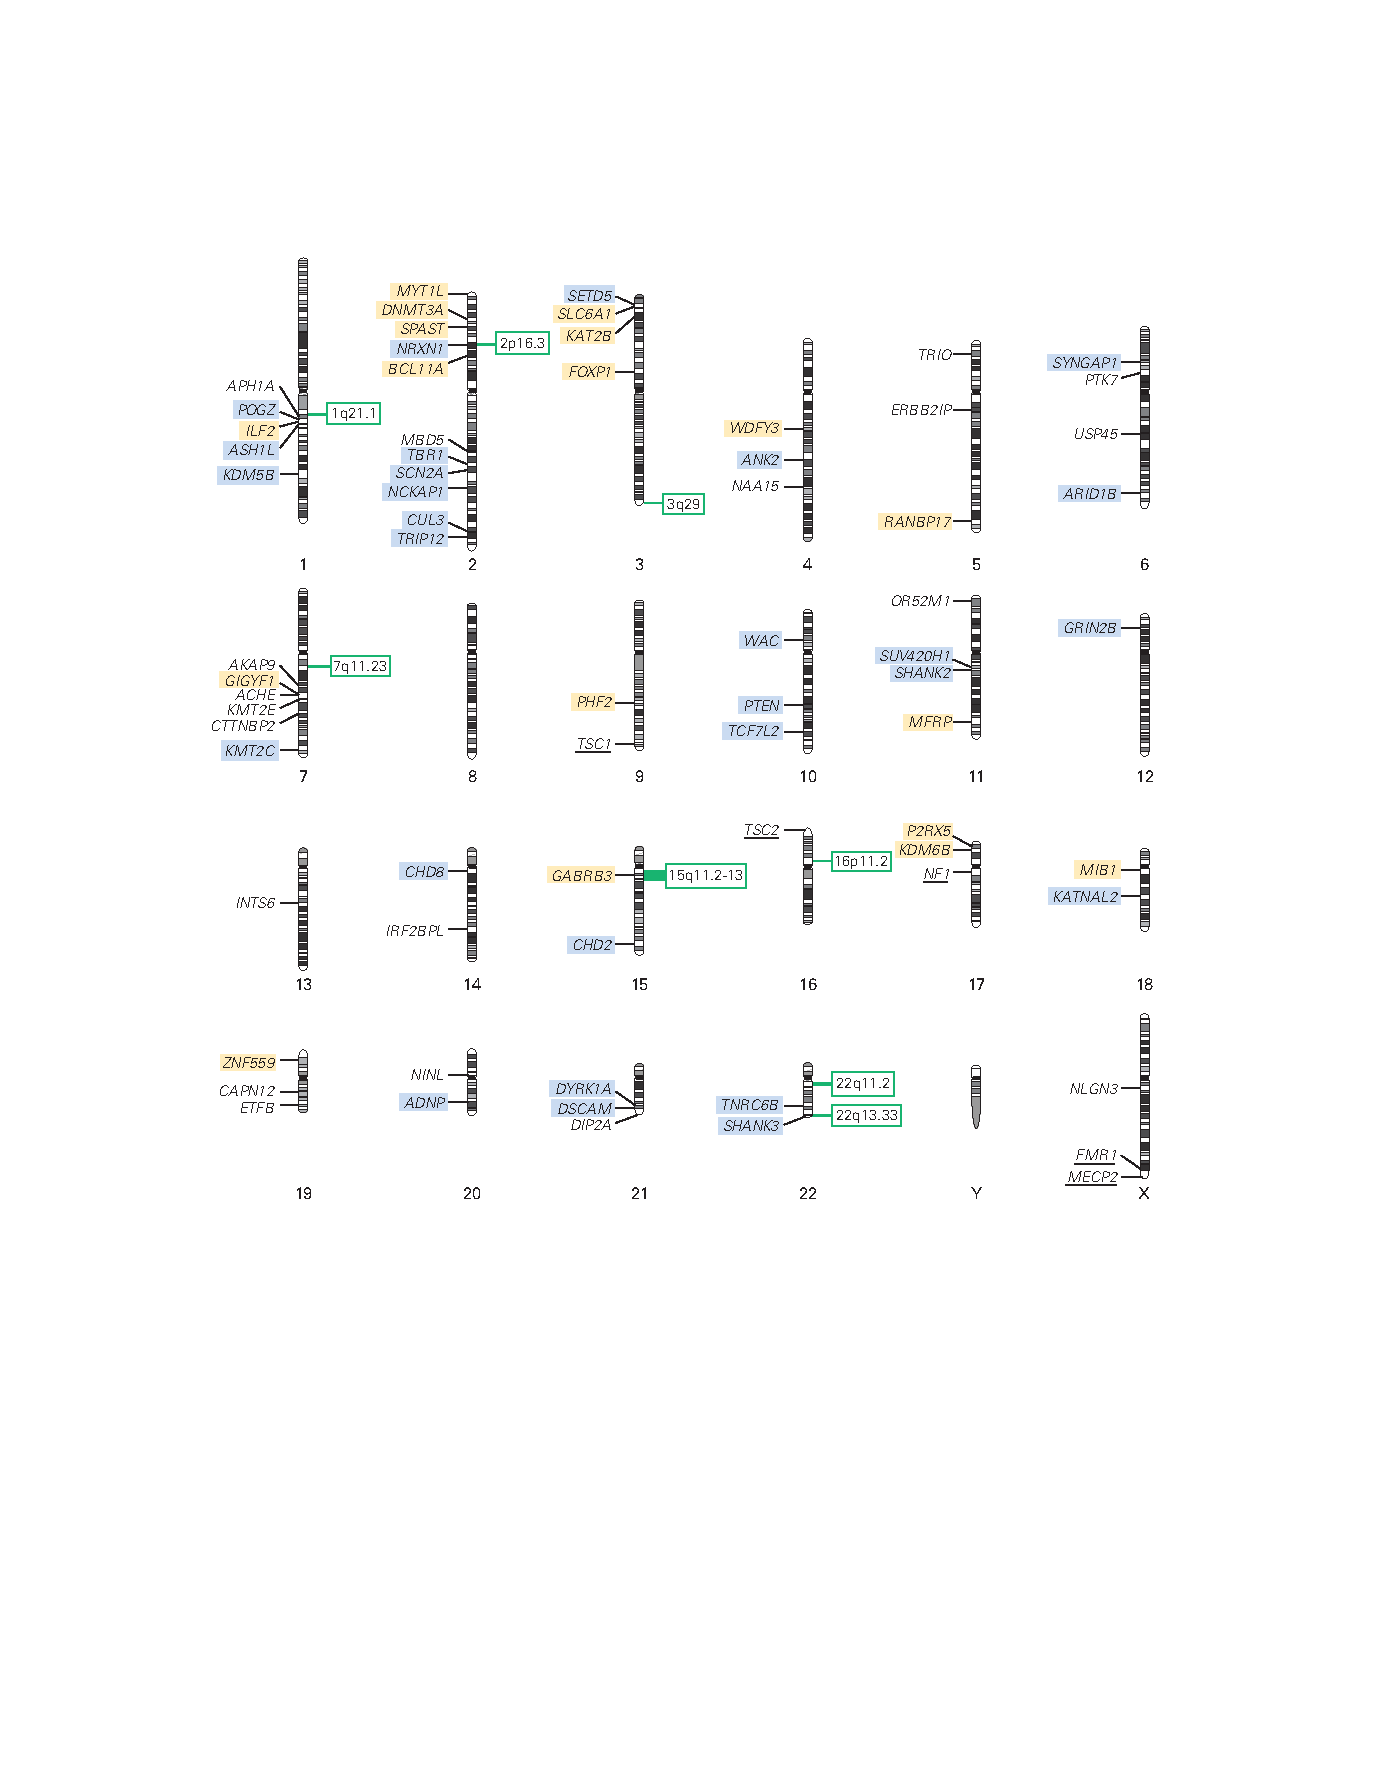
\includegraphics[width=0.9\linewidth]{chap62/fig_62_8}
	\caption{Prader-Willi 和 Angelman 综合症的印记。 大约 70\% 的 Prader-Willi 和 Angelman 综合征患者从一位父母那里继承了 15 号染色体,并伴有 q11-13 间期的自发性(非遗传性)缺失。 该间隔包含带有等位基因的印迹基因,这些等位基因的表达或不表达取决于染色体是从父亲还是母亲遗传的。 如果缺失的染色体来自父亲,则会出现普瑞德-威利综合症,因为在完整母体染色体的相应区间(例如基因 B)上的母体印记基因未表达。 如果缺失的染色体来自母亲,则泛素连接酶基因(UBE3A)由于印记作用在父本染色体上正常失活,因此不会在后代中表达; 该基因表达的缺失会导致 Angelman 综合征。}
	\label{fig:62_8}
\end{figure}


从头突变的研究在本千年的第二个十年取得了进展,导致发现与从头拷贝数变异相似,DNA 序列的从头变化——包括单核苷酸变异和插入或缺失 (indels)—— 也有助于 ASD 风险,并且可以类似地用于识别特定的风险基因。
最近的报告现在已经利用这种方法来包括 100 多个携带大效应单核苷酸变异和插入缺失突变的基因,这些突变会破坏编码蛋白的功能(即可能的基因破坏性 [LGD] 突变)(第 \ref{chap:chap2} 章)。


这里值得一提的是几个相关的发现。
首先,尽管从头突变对总人口中 ASD 风险的贡献很小(在 3\% 左右),但在临床环境中发现并招募的具有大效应从头突变的个体比例 基因研究相当显着,女孩高达40\%。 造成这种明显矛盾的原因是,对人口而言,大部分风险都是以影响较小的常见变异形式进行的,这些变异在大多数人中不足以导致他们超过 ASD 的诊断阈值。
简而言之,人群中大多数携带某种程度风险的人从未表现出明显的社交障碍,也没有引起临床关注。
相反,具有大效应从头拷贝数变异、单核苷酸变异和插入缺失的个体更有可能出现明显的临床表现并寻求医疗救助。


其次,使用外显子组测序对 ASD 中的从头单核苷酸变异和插入缺失进行的研究发现,从头突变的发生率随着父亲的年龄而增加。
与这一观察结果一致的是,ASD 病例中绝大多数有害的从头序列突变都存在于父系遗传的染色体上。
尽管风险随年龄增长的绝对增加很小,但这一观察结果仍然为理解 ASD 患病率的长期增加提供了一个概念框架。
它还为进一步研究环境因素对增加从头突变的影响,从而可能增加临床 ASD 病例的真实发病率奠定了基础。


从头大效应突变与智力障碍的关系一直是大量讨论的主题,一些人认为从头大效应突变通常见于患有智力障碍的 ASD 中。
尽管具有破坏性的从头突变(拷贝数变异或单核苷酸变异)在 IQ 较低的 ASD 患者中更为普遍,但在整个 IQ 范围内也发现了赋予 ASD 风险的突变 ,强化了认知和社会功能领域在某种程度上是可分离的观点。


ASD 的遗传学与其他常见疾病(包括精神分裂症)之间的一个显着差异是使用全基因组关联研究缺乏进展(第 \ref{chap:chap2} 章)。
迄今为止,仅发现了少数与 ASD 风险显着且可重复相关的常见遗传变异。
此外,由于缺乏全基因组关联研究的结果,以及这些关联源自一种方法 凭经验证明在复杂的常见疾病中发现基因是不可靠的。
另一方面,如前所述,有非常有力的证据表明,共同变异在 ASD 人群风险中起着重要作用。
事实上,已经推断出这种变异的贡献程度的全基因组关联研究一致认为,大部分的脆弱性存在于共同变异中。
人们可以通过注意到那些显着损害生殖健康的疾病(例如自闭症谱系障碍)来调和这些观察结果,只有携带小影响的常见遗传变异会在许多代人中保留下来。
那些影响较大的将要么被驱动到低频率,要么被自然选择完全移除。
此外,迄今为止,ASD 的病例对照全基因组关联研究的样本量比那些在识别与精神分裂症相关的常见多态性方面取得显着成功的样本量要小。
简而言之,有限的能力几乎肯定是识别导致 ASD 的常见小效应等位基因的关键限制。


在识别从头突变方面的相对成功并不表明这些是 ASD 风险的唯一重要机制。
该领域的最新进展是突变的大效应大小、它们位于基因组最容易解释的部分(编码区)以及它们在典型发育个体中的低碱基率的偶然组合的结果。
然而,就人群风险而言,与罕见的高效变异相比,常见的非编码、小效应等位基因可能共同占 ASD 责任的更大比例。
此外,还有隐性形式的 ASD 的证据。
这些最初主要是通过鉴定纯合子功能丧失突变(即父系和母系遗传染色体上的相同破坏性等位基因)在近亲种群中鉴定出来的,包括基因 CNTNAP2、BCKDK 和 NHE9。
此外,最近的几项研究强调了复合杂合子突变对 ASD 风险的贡献——即,在低血缘关系人群中,不同突变映射到母系和父系遗传染色体上的同一基因。


一个关键点是,追求和发现不同类型的突变可能有助于以不同的方式推进科学。
例如,可以在模型系统中快速研究罕见的从头产生的高效突变。
此外,常见变异提供了评估研究队列总体多基因风险的机会,这种方法可能对多模式研究非常有用,例如将神经影像与遗传数据相结合的研究,或将人类行为与基因型联系起来的其他研究。
最后,非常罕见的纯合/隐性变异减轻了单倍体不足建模的一些挑战。


尽管遗传力——由于遗传因素导致的表型变异的比例——对于 ASD 来说非常高,但环境因素也发挥了作用,尽管很少有特定的环境因素被最终确定。
子宫内病毒(如风疹、麻疹、流感、单纯疱疹病毒和巨细胞病毒)感染可能导致 ASD 的病因。
有大量证据表明,免疫功能的介质也在大脑发育(包括突触形成)中发挥作用。
鉴于 ASD 的复杂性及其多种形式,最终可能会发现多种病因——一些是纯遗传性的,另一些取决于遗传风险因素和环境因素的组合,还有一些是纯粹的环境原因。



\section{遗传学和神经病理学正在阐明自闭症谱系障碍的神经机制}

\subsection{可以使用系统生物学方法解释遗传发现}

基因发现的最新进展是一个特别令人兴奋的发展,为使用越来越多的体外和体内方法进行生物分析提供了许多机会。
此外,当代基因组方法同时检查基因组的大部分,允许在风险基因组的研究中使用无偏见的方法,以努力确定不同 ASD 基因之间的聚合点。


迄今为止,检查多个系统的生物学方法大致分为两种类型的努力:
一种是试图确定不断增长的 ASD 基因列表中反映的生物过程类型,另一种是试图确定生物过程的汇聚点 分子或细胞水平。
后一种方法基于这样一种观念,即不同途径中的多种类型的遗传驱动扰动可能导致共同的表型,因为它们在人脑发育过程中的特定时间点在特定细胞类型、区域或回路上趋同。


在零假设下,ASD 风险基因的比例高于预期的生物过程或途径包括染色质修饰、突触功能、WNT 信号通路和 FMRP 的靶标。
这份清单显然并不详尽。
例如,我们从涉及遗传综合征的基因以及导致非综合征或特发性 ASD 的基因中了解到,突触局部蛋白质合成和神经发生是不同风险突变的潜在生物学汇聚点。


这些发现中的一些差异几乎可以肯定是由于 ASD 风险基因的不同选择标准以及用于注释其功能的数据的差异。
后一个问题很重要,因为在当前注释分配给给定基因或蛋白质的生物过程的努力中存在许多混杂因素。
这些包括数据来源。
例如,一个基因的指定功能可能会受到发表偏倚的显着影响,无论是采用体外还是体内试验,以及使用什么类型的组织和模型系统来生成数据。
此外,大多数功能注释提供的有关基因功能时间进程的信息有限,这些基因可能受发育调节和生物多效性。
尽管如此,最引人注目的是研究结果的一致性不断提高。
尽管方法各不相同,但上述生物过程已在各种严格的研究中反复确定。


如前所述,确定多个自闭症风险基因重叠位置的另一种方法不仅包括检查它们的功能,还包括检查它们的发育表达模式。
此类研究基于这样的概念,即多个风险基因可能具有不同的明显功能,但具有破坏相同回路、细胞或发育过程的能力。
例如,编码已知介导突触粘附的蛋白质的基因突变和编码染色质修饰基因的单独突变都可能导致早期皮质纹状体连接发育的相同异常。
在这种情况下,扰动的时间和位置可能与特定分子途径或单个基因的指定分子功能一样相关。
这些研究也倾向于依赖于检测全基因组的发育表达轨迹,以最大限度地减少与其他可用注释系统相关的一些混杂因素。
例如,现在基本上可以同时检测基因组中的每个基因——无需依赖先前的研究来为基因分配特定功能。
此外,此类研究越来越多地检查人类和/或非人类灵长类动物大脑中的基因表达,从而减轻了依赖体外数据的一些挑战。
当然,此类研究仍必须应对表达分析的分辨率限制以及不同大脑区域的不完整(且可能有偏见)的表示。
尽管如此,迄今为止,不同研究之间的一致性程度令人欣慰。


尽管在这些类型的研究中使用的分析和统计方法存在差异,但迄今为止普遍认为 ASD 风险基因指向人类中期胎儿皮质发育的脆弱性。
还有新出现的证据表明,这些基因指向大脑皮层以及纹状体和小脑中的深层和上层投射神经元的参与(尽管与皮层区域相比,这些区域的发育表达数据在可公开访问的数据库中仍然有限)。



\subsection{自闭症谱系障碍基因已在多种模型系统中得到研究}

由于最近取得了巨大进展,即使是对动物模型中 ASD 研究文献的粗略描述也超出了本章的范围。
在某种程度上,这是研究数量庞大的结果; 在某种程度上,它是所研究扰动类型显着差异的产物(例如,经过充分验证的遗传模型、“候选基因”模型、药理学模型,如丙戊酸盐暴露或母体免疫激活)。
此外,大脑区域、细胞类型、发育时期和所检测的生物过程的差异使得概括概括存在问题。
简而言之,关于与 ASD 相关的病理生理机制的范围尚未达成共识。


尽管如此,鉴于人类遗传学的最新进展,区分基于可重复遗传发现的模型(包括导致综合征性 ASD 的模型)和基于不可靠候选基因位点或仅基于行为(即那些似乎可以复制的行为)的模型变得越来越重要 人类症状)。
鉴于现在有多种选择可用于研究在感兴趣的表型中明显增加人类患 ASD 风险的遗传变异,研究与人类病理生理学具有更微弱联系的模型越来越难以证明其合理性。


许多报告 ASD 啮齿动物模型的出版物,无论其起源如何,都关注与人类综合征中所见症状相似的表型,包括社交互动、发声和让人联想到人类焦虑或攻击行为的变化。 即使偏向于发表积极的发现,结果也会有很大差异。
值得注意的是,鉴于人类与最常用的实验动物在大脑发育、组织和功能方面的重要差异,长期以来一直存在关于 ASD 动物模型相关性的争论。
然而,对广泛的动物行为进行公正的评估——不一定优先考虑那些“看起来”像核心 ASD 症状的行为——很可能为了解病理生理机制提供一个有价值的窗口。
例如,迄今为止,各种 ASD 遗传模型(以及各种实验室)报告的一些最常见的表型涉及运动行为。
在这种情况下,观察到的行为是否让人联想到人类的核心诊断特征似乎远不如观察表明生物融合的重要点重要,为 ASD 涉及的细胞类型、回路和过程提供线索。


尽管啮齿动物模型继续主导 ASD 文献,但范围广泛的其他模型已经提供了对生物学的重要见解。
这些包括果蝇、蠕虫、斑马鱼、青蛙、田鼠、非人类灵长类动物、诱导多能干细胞和脑类器官,以及人类尸检样本。
鉴于手头问题的复杂性、各种模型的不同优势和局限性以及不同物种大脑结构和发育的重要差异,持续的进步可能需要整合各种现有模型的数据,从苍蝇和蠕虫到 人类。



\subsection{尸检和脑组织研究提供了对自闭症谱系障碍病理学的洞察力}

自闭症在微观层面的神经病理学也尚不清楚,但一些研究提供了多种解剖学相关性的可能性的证据。
多重相关可能部分是由于可用于病理分析的大脑数量较少。
此外,其中只有一小部分进行了定量分析。 另一个问题是癫痫病的频繁发生。
大约 30\% 的自闭症患者也有癫痫症,癫痫发作可能会损害杏仁核和许多其他与 ASD 相关的大脑区域。


ASD 最早和最一致的解剖学发现之一是某些个体小脑中浦肯野细胞数量较少。
当神经染色剂用于标记细胞体时,浦肯野细胞有序排列中的间隙是显而易见的。
这种细胞数量的减少是因为自闭症谱系障碍、癫痫,还是这两种疾病的同时发生,目前尚不清楚。
还不清楚浦肯野细胞数量的减少是否特别是 ASD 或更普遍的神经发育障碍的特征。
在特发性智力障碍、Williams 综合征和其他神经发育障碍病例中发现了各种各样的小脑变化。
还报道了一些与小脑相连的脑干核团改变的病例,例如橄榄复合体。
最后,当代分析发现细胞数量存在相当大的异质性,只有一部分样本显示浦肯野细胞数量减少。


在自闭症大脑皮层中也观察到了微观异常,包括细胞迁移到皮层中的缺陷,例如异位(白质中未能进入皮层的细胞巢)。
也有人提出自闭症皮层的柱状组织异常。
这些发现仍在等待使用定量策略的更大规模研究的证实。
最后,一项研究发现没有癫痫的自闭症患者成熟杏仁核中的神经元较少。


在对来自 ASD 患者的活体病理组织样本(在顽固性癫痫手术期间从三名患者身上取出)的少数报告描述之一中,在颞叶皮质中发现了多种细胞结构异常。
这些个体都在基因接触蛋白相关蛋白样 2 中携带罕见的隐性功能丧失突变。在这些患者中观察到多种组织学异常,包括皮质增厚区域和灰质与白质之间的边界模糊。
此外,作者描述了多个皮层区域中的神经元异常组织成紧密排列的柱状或簇状。
在海马体和颞叶皮层中,神经元的数量都增加了,并且许多神经元的形状异常,而不是它们的锥体形态。
鉴于三名患者中有两名在 MRI 上可见明显的颞叶异常、罕见的隐性遗传贡献以及特别严重的癫痫发作,这些发现对特发性 ASD 的普遍性仍然存在疑问。


一些 ASD 患者存在神经解剖学变化的总体观点得到了其他几条证据的支持。
许多得到充分支持和充分表征的 ASD 风险基因(例如,PTEN 突变)与大脑大小的增加有关,范围从适度(例如,CHD8 功能丧失突变)到明显的巨头畸形。
此外,自闭症谱系障碍通常与小头畸形有关。
患有 Rett 综合征的女孩会出现小头畸形,这毫不奇怪地表明,社会残疾表型可能会出现多种解剖学紊乱。



\section{基础科学和转化科学的进展为阐明自闭症谱系障碍的病理生理学提供了途径}

全面了解导致社会和智力障碍的许多神经发育障碍的神经生物学基础需要神经科学、其他医学学科、计算生物学和基因组学的融合。
自下而上的方法——从识别导致认知和行为障碍的基因到了解它们对大脑发育的影响——已经提供了一些关键的见解。
同时,通过识别和定义涉及社会功能和功能障碍的关键神经回路,自上而下的方法也可能非常有效。


幸运的是,可用于追求这两种方法的工具越来越容易获得,从高通量全基因组测序到快速推进的信息学管道、基因组编辑、光遗传学和其他研究体内回路的方法、单细胞技术、改进的神经成像方法和技术,以及 开发易于处理的人类和非人类灵长类动物神经模型,包括大脑类器官。


尽管在阐述 ASD 和其他神经发育障碍的遗传学和生物学方面取得了很大进展,但基因组研究的结果也指出了一些关键挑战:
在最基本的层面上,将这些发现转化为对病理生理学的理解是有限的 根据目前关于大脑组织和发育的知识状况。
如果不对人类、非人类灵长类动物和其他模型系统的大脑进行详细的细胞理解,那么解释各种各样的遗传扰动并从对生物学的理解转变为对发病机制的任何理解将是具有挑战性的。
也有理由假设,为了对本章讨论的这类疾病最有用,这种类型的地图必须捕捉发展维度。
令人兴奋和振奋的是,最近的 BRAIN 计划、其他大规模的政府努力以及私人基金会的努力都强调基础知识是成功的关键。


毫无疑问,一方面我们的临床现象学、遗传学、影像学和神经病理学知识与另一方面将深刻改善严重受影响个体生活的新疗法的发展之间的距离似乎令人望而生畏。
同时,看到孟德尔神经发育障碍的进展令人振奋,一些理性疗法的临床试验已经完成,而其他的临床试验正在进行中。
尽管一些早期结果令人失望,但对这些综合症的理解已经发展到这一点这一事实本身就足以让人保持乐观。
按照这些思路,考虑本章从前一卷到当前卷所需的修订范围是很有用的。
自信地在近 100 个基因组位点和基因中分配大效应遗传风险的能力、关于涉及哪些类型的分子过程和途径的新共识、对发育特征的初步了解以及生物学驱动的治疗试验的启动都已经成为现实。
在相对较短的时间内出现。 令人兴奋的是,随着本书下一次修订的出版,这个领域可能会出现在哪里。



\section{亮点}

1. 神经发育综合症可能涉及不同认知领域的不同程度的损害。
涉及社会领域功能障碍的综合症,无论是否涉及一般认知或知觉,都是本章的重点。


2. 自闭症是典型的社会残疾综合症,Leo Kanner 于 1943 年在文献中首次对其进行了描述。
今天,自闭症被认为是一系列具有两个定义诊断特征的障碍:
社交沟通受到根本损害和刻板行为和/或兴趣高度受限。
据估计,自闭症谱系障碍 (ASD) 在发达国家的患病率至少为 1.5\%,男性患病率远高于女性。


3. 环境因素和无数基因都会导致 ASD 风险。
这种遗传复杂性导致几十年来在绘制特定 ASD 风险基因和基因组区域(基因座)方面的努力进展甚微。


4. ASD 遗传学和神经生物学的最早线索来自对同时表现为智力障碍和社会障碍的神经发育综合征的早期调查。
其中包括脆性 X 综合征、Rett 综合征、Williams 综合征以及 Prader-Willi 和 Angelman 综合征。 


5. 高通量基因组技术、大量患者队列的整合以及对 ASD 研究的大量投资已经改变了特发性 ASD 基因发现领域。
目前,已有数十个特定基因和基因组区域可靠且可重复地与 ASD 风险相关联。 


6. 常见类型 ASD 遗传学的最新进展源于对基因组编码部分罕见和偶发(从头)突变的关注。
平均而言,这些突变带来的生物学效应比在其他精神疾病研究中发现的要大得多,例如精神分裂症,在精神分裂症中已经发现了许多常见的遗传风险变异,每个变异都有很小的影响。


7. 对遗传综合征和特发性 ASD 的研究已经开始揭示病理生理学中涉及的过程、途径和发育时期。
这些包括表观遗传机制和染色质动力学、突触功能障碍以及异常局部蛋白质合成的作用。
最近对基因决定的 ASD 的研究也表明,人类中期胎儿皮质发育和谷氨酸能神经元特别脆弱。


8. 目前可获得大量经证实的 ASD 位点,包括综合征型和特发性病症,为神经生物学研究提供了坚实的基础。
这些进展提供了与人类病理生理学的紧密联系,包括在因果关系问题上的潜在牵引力,因为种系遗传变化在大脑发育的最早阶段就已经存在。


9. 除了提供有关特发性 ASD 分子机制的一些初步线索外,孟德尔综合征的研究还通过强调发育表型的潜在可逆性来挑战传统智慧。
这些观察结果,特别是关于 Rett 综合征和脆性 X 综合征的观察结果,使人们对合理开发治疗方法的机会产生了新的乐观情绪。


10. 目前正在融合多种方法来阐述 ASD 的病理学,包括基因发现和系统生物学、模型系统方法、神经影像学研究和神经病理学研究。
未来的主要挑战将是从对生物学的一般理解转变为对病理生理学的可操作理解。

